\graphicspath{{./figures/}}
\title{bounds checking (2) / testing (1)}
\date{}
\begin{document}
\begin{frame}
    \titlepage
\end{frame}

\begin{frame}{last time}
    \begin{itemize}
    \item use-after-free vulnerabilities
        \begin{itemize}
        \item after free: old pointer still ``works'' if new thing allocated there
        \item attacker can get control of memory of object they didn't use
        \item info leak (read from object you shouldn't)
        \item code execution (replace VTable/function pointer/etc.)
        \end{itemize}
    \item FORTIFY\_SOURCE: gcc/clang/etc.'s sometimes bounds checking
        \begin{itemize}
        \item special \texttt{chk} version of library functions
        \item works when compilers can find bounds easily
        \item compiler can't find bounds: no fallback
        \end{itemize}
    \item unfortunate design of strncpy, strncat
    \end{itemize}
\end{frame}

\usetikzlibrary{arrows.meta,calc,patterns}
% fIXME: overflow
\section{bounds checking...}
\subsection{and library functions}
        % FIXME: exercise: what should call have been
            % needs answers

\begin{frame}[fragile,label=nonChecking]{non-checking library functions}
\lstset{language=C,style=small}
    \begin{itemize}
    \item some C library functions make bounds checking hard: 
\begin{lstlisting}
strcpy(dest, source);
strcat(dest, source);
sprintf(dest, format, ...);
\end{lstlisting}
    \item bounds-checking versions (\myemph{added to library later}):
\begin{lstlisting}
/* might not add \0 (!) */
strncpy(dest, source, size);
strncat(dest, source, size);
snprintf(dest, size, format, ...);
\end{lstlisting}
    \end{itemize}
\end{frame}

\begin{frame}[fragile,label=poorBoundsChecking]{poor bounds-checking APIs}
\begin{lstlisting}[language=C,style=smaller]
char dest[100];
/* THIS CODE IS BROKEN */
strncpy(dest, source1, sizeof dest);
strncat(dest, source2, sizeof dest);
printf("result was %s\n", dest)
\end{lstlisting}
\begin{itemize}
\item the above can access memory of out of bounds
\item \ldots in a bunch of ways
\end{itemize}
\end{frame}

\begin{frame}[fragile,label=strncpyManual]{Linux's strncpy manual}
\begin{lstlisting}[language=C,style=smaller]
strncpy(dest, source1, sizeof dest);
\end{lstlisting}
\begin{itemize}
\item ``Warning: If there is no
       null byte among the first n bytes of src, the string placed in dest will not be null-terminated.''
\end{itemize}
\begin{itemize}
\item exercise: what should the call have been?
\end{itemize}
\end{frame}


\begin{frame}[fragile,label=strncatManual]{Linux's strncat manual}
\begin{lstlisting}[language=C,style=smaller]
strncat(dest, source2, sizeof dest);
\end{lstlisting}
\begin{itemize}
\item ``If src contains n or more bytes, strncat() writes n+1 bytes to  dest  (n
from  src  plus the terminating null byte).  Therefore, the size of dest
must be at least strlen(dest)+n+1.''
\end{itemize}
\begin{itemize}
\item exercise: what should the call have been?
\end{itemize}
\end{frame}

\begin{frame}[fragile,label=betterStrX]{better versions?}
\begin{itemize}
\item FreeBSD (and Linux via libbsd): strlcpy, strlcat
\item ``Unlike [strncat and strncpy], strlcpy() and strlcat() take the full size of the buffer
        and gaurenteeto NUL-terminate the result...''
\end{itemize}
\begin{lstlisting}[language=C++,style=smaller]
strlcpy(dest, source1, sizeof dest);
strlcat(dest, source2, sizeof dest);
\end{lstlisting}
\vspace{.5cm}
\begin{itemize}
\item Windows: \texttt{strcpy\_s}, \texttt{strcat\_s} (same idea, differentname)
\end{itemize}
\end{frame}

\begin{frame}[fragile,label=cppBounds]{C++/Rust bounds checking}
\lstset{language=C,style=small}
\begin{lstlisting}
#include <vector>
...
std::vector<int> data;
data.resize(50);
// undefined behavior:
data[60] = 0;
// throws std::out_of_range exception
data.at(60) = 0;
\end{lstlisting}
\vspace{-\baselineskip}
\hrulefill
\begin{Verbatim}[fontsize=\small]
let data: Vec<i32> = ...;
data.resize(50, 0);
// undefined behavior:
unsafe { *data.get_unchecked_mut(60) = 1; }
// panics at runtime:
data[60] = 0;  
\end{Verbatim}
\end{frame}



\subsection{language support?}


\begin{frame}{language-level solutions}
    \begin{itemize}
    \item languages like Python don't have this problem
    \item couldn't we do the same thing in C?
    \end{itemize}
\end{frame}




\subsection{simple case for bounds checking in C}
\begin{frame}{bounds-checking C}
    \begin{itemize}
    \item there have been many proposals to add bounds-checking to C
    \item including implementations
    \item brainstorm: \myemph{why hasn't this happened?}
    \end{itemize}
\end{frame}

\begin{frame}[fragile,label=addBounds]{easy bounds-checking}
    \lstset{language=C,style=smaller}
\begin{lstlisting}
void vulnerable() {
    char buffer[100];
    int c;
    int i = 0;
    while ((c = getchar()) != EOF && c != '\n') {
        buffer[i] = c;
    }
}
void vulnerable_checked() {
    char buffer[100];
    int c;
    int i = 0;
    while ((c = getchar()) != EOF && c != '\n') {
        FAIL_IF(i >= 100 || i < 0);
        buffer[i] = c;
    }
}
\end{lstlisting}
\end{frame}


\subsection{the problematic case}
\begin{frame}[fragile,label=addBoundsHarder]{harder bounds-checking}
    \lstset{language=C,style=smaller}
\begin{lstlisting}
void vulnerable(char *buffer) {
    char buffer[100];
    int c;
    int i = 0;
    while ((c = getchar()) != EOF && c != '\n') {
        buffer[i] = c;
    }
}
void vulnerable_checked(char *buffer) {
    int c;
    int i = 0;
    while ((c = getchar()) != EOF && c != '\n') {
        FAIL_IF(i >= UNKNOWN || i < UNKNOWN);
        buffer[i] = c;
    }
}
\end{lstlisting}
\end{frame}


\subsection{fat pointer idea}
% FIXME: smoother transition
    % FIXME: exercise about problematic cases


\begin{frame}[fragile,label=wrappedPointers]{adding bounds-checking --- fat pointers}
\lstset{
    language=C,
    style=small
}
\begin{lstlisting}
struct MyPtr {
    char *pointer; /* "raw" pointer value */
    char *minimum; /* first byte of buffer pointed to */
    char *maximum; /* last byte of buffer pointed to */
};
\end{lstlisting}
\begin{visibleenv}<2->
\hrule
\begin{lstlisting}
char buffer[100];
char *p = &buffer[10];
\end{lstlisting}
becomes
\begin{lstlisting}
char buffer[100];
MyPtr p = {
    .pointer = &buffer[10],
    .minimum = &buffer[0],
    .maximum = &buffer[99]
};
\end{lstlisting}
\end{visibleenv}
\end{frame}



\subsubsection{strcpy example}
\begin{frame}[fragile,label=wrappedPtrStrcpy]{adding bounds checking --- strcpy}
\lstset{
    language=C,
    style=small
}
\begin{lstlisting}
MyPtr strcpy(MyPtr dest, const MyPtr src) {
    int i;
    do {
        CHECK(src.pointer + i <= src.maximum);
        CHECK(src.pointer + i >= src.minimum);
        CHECK(dest.pointer + i <= dest.maximum);
        CHECK(dest.pointer + i >= dest.minimum);
        dest.pointer[i] = src.pointer[i];
        i += 1;
        CHECK(src.pointer + i <= src.maximum);
        CHECK(src.pointer + i >= src.minimum);
    } while (src.pointer[i] != '\0');
    return dest;
}
\end{lstlisting}
\end{frame}




\subsubsection{overhead?}

\begin{frame}{speed of bounds checking}
    \begin{itemize}
    \item two comparisons for every pointer access?
    \item three times as much space for every pointer?
    \end{itemize}
\end{frame}



\subsection{unfortunate things C programmers do}
\begin{frame}[fragile,label=unfortunateCProg1]{unfortunate things C programmers do (1)}
from FreeBSD's bootpd (server for machines that boot from the network):
\begin{lstlisting}[language=C,style=smaller]
struct shared_string {
    unsigned int linkcount;
    char         string[1]; /* Dynamically extended */
};
...
s = (struct shared_string *) smalloc(
        sizeof(struct shared_string) + length
    );
...
\end{lstlisting}
\end{frame}

\begin{frame}[fragile,label=unfortunateCProg2]{unfortunate things C programmers do (2)}
from perl's source code:
\begin{lstlisting}[language=C,style=small]
sv_setuv(my_pool_sv, PTR2UV(my_poolp));
...
/* later, in another function: */
my_pool_t *my_poolp = INT2PTR(my_pool_t*, SvUV(my_pool_sv));
\end{lstlisting}
\begin{itemize}
\item PTR2UV: pointer to Unsigned int Value
\item INT2PTR: integer to pointer value
\end{itemize}
\end{frame}

\begin{frame}[fragile,label=unfortunateCProg3]{unfortunate things C programmers do (3)}
\begin{lstlisting}[language=C,style=small]
struct SuperClass;
struct SubClass {
    struct SuperClass super;
    ...
}

struct SubClass sub;
struct SuperClass *super = &sub.super;
some_function(super);
...
some_function(struct SuperClass *super) {
    ...
    struct SubClass *sub = (struct SubClass *)super;
    ...
}
\end{lstlisting}
\end{frame}



\subsection{fat pointers in reality?}
\begin{frame}{example: CCured}
\begin{itemize}
\item Necula et al, ``CCured:  Type-Safe Retrofitting of Legacy Code'' (2002)
\vspace{.5cm}
\item extension to C to add fat pointers
\item actually three different types of pointers:   
    \begin{itemize}
    \item SAFE: point to single object (not array) or NULL
    \item SEQUENCE: pointer to array with known bounds (like ``fat'' pointers)
    \item DYNAMIC: extra to handles type-casting
    \end{itemize}
\item \textit{needs source changes} to annotate some pointer usage
    \begin{itemize}
    \item especially to allow library function calls
    \end{itemize}
\item 1-\textbf{2.5x} time overhead
\end{itemize}
\end{frame}


\section{baggy bounds checking}

\begin{frame}{research example (2009)}
    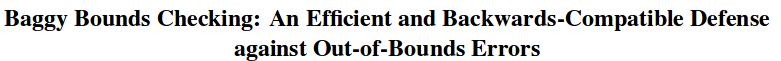
\includegraphics[width=\textwidth]{../bounds/baggy-bounds-title}
\end{frame}

\begin{frame}[fragile,label=lookupTable]{baggy bounds checking idea}
    \begin{itemize}
        \item giant lookup table --- one entry for every 16 bytes of memory
        \item table indicates start of object allocated here
        \item check pointer arithmetic:
    \end{itemize}
\begin{lstlisting}
char p = str[i];
/* becomes: */
CHECK(START_OF[str / 16] == START_OF[&str[i] / 16]);
char p = str[i];
\end{lstlisting}
\end{frame}




\subsection{trick for good performance}

\begin{frame}[fragile,label=baggyBoundsTrick]{baggy bounds trick}
\lstset{language=C,style=small}
    \begin{itemize}
        \item table of pointers to starting locations would be huge
        \item add some restrictions:
            \begin{itemize}
            \item all object sizes are powers of two
            \item all object starting addresses are a multiple of their size
            \end{itemize}
        \item then, table contains size info only:
            \begin{itemize}
            \item table contains $i$, size is $2^i$ bytes:
            \end{itemize}
    \end{itemize}
\begin{lstlisting}
char *GetStartOfObject(char *pointer) {
    return pointer & ~(1 << TABLE[pointer / 16] - 1);
    /* pointer bitwise-and 2^(table entry) - 1 */
    /* clear lower (table entry) bits  of pointer */
}
\end{lstlisting}
\end{frame}



\subsection{the lookup table}
\usetikzlibrary{fit,matrix}

\tikzset{
    stackBox/.style={very thick},
    allocBox/.style={dashed,very thick,fill=blue!20},
    onStack/.style={thick},
    frameOne/.style={fill=blue!15},
    frameTwo/.style={fill=red!15},
    markLine/.style={blue!50!black},
    markLineB/.style={red!90!black},
    hiLine/.style={red!90!black},
}
\begin{frame}<1-6>[fragile,label=lkpTble]{allocations and lookup table}
    \begin{tikzpicture}
        \draw[onStack] (0, 0) rectangle (4, -7);
        \draw[allocBox] (0, 0) rectangle (4, -0.4);
        \draw[stackBox] (0, 0) rectangle (4, -0.5);
        \draw[allocBox] (0, -0.5) rectangle (4, -0.8);
        \draw[stackBox] (0, -0.5) rectangle (4, -1.0);
        \draw[allocBox] (0, -1) rectangle (4, -1.9);
        \draw[stackBox] (0, -1) rectangle (4, -2);
        \draw[allocBox] (0, -2) rectangle (4, -2.4);
        \draw[stackBox] (0, -2) rectangle (4, -2.5);
        \draw[allocBox] (0, -2.5) rectangle (4, -2.7);
        \draw[stackBox] (0, -2.5) rectangle (4, -3);
        \draw[stackBox] (0, -3) rectangle (4, -4);
        \draw[allocBox] (0, -4) rectangle (4, -5.2);
        \draw[stackBox] (0, -4) rectangle (4, -6);

        \begin{visibleenv}<1->
            \node[anchor=north west,align=left] at (9, 0) {
                object allocated in \\ \myemph<1>{power-of-two `slots'}
            };
        \end{visibleenv}
        \begin{visibleenv}<2->
            \matrix[tight matrix,
                nodes={text width=1cm,font=\small\tt},anchor=north west,label={north:table}] (tbl) at (7, -1) {
                $2^4$ \\ $2^4$  \\ $2^5$ \\ $2^5$ \\ $2^4$ \\ $2^4$ \\
                $0$ \\ $0$ \\
                $2^6$ \\ $2^6$ \\ $2^6$ \\ $2^6$ \\
            };
            \begin{scope}[thick,dotted,-Latex]
            \draw (4, -.25) -- (tbl-1-1.west);
            \draw (4, -.75) -- (tbl-2-1.west);
            \draw (4, -1.25) -- (tbl-3-1.west);
            \draw (4, -1.75) -- (tbl-4-1.west);
            \draw (4, -2.25) -- (tbl-5-1.west);
            \draw (4, -2.75) -- (tbl-6-1.west);
            \draw (4, -3.25) -- (tbl-7-1.west);
            \draw (4, -3.75) -- (tbl-8-1.west);
            \draw (4, -4.25) -- (tbl-9-1.west);
            \end{scope}
        \end{visibleenv}
        \begin{visibleenv}<3>
            \draw[ultra thick,red] (0, -1) rectangle (4, -2);
            \node[draw,ultra thick,red,inner sep=0mm,fit=(tbl-3-1) (tbl-4-1)] {};
            \draw[ultra thick,blue] (0, -4) rectangle (4, -6);
            \node[draw,ultra thick,blue,inner sep=0mm,fit=(tbl-9-1) (tbl-12-1)] {};
        \end{visibleenv}
        \begin{visibleenv}<3->
            \node[anchor=north west,align=left] at (9, -2) {
                table stores sizes \\
                \myemph{for each 16 bytes}
            };
        \end{visibleenv}
        \begin{visibleenv}<4>
            \draw[ultra thick,red] (0, -3) rectangle (4, -4);
            \node[draw,ultra thick,red,inner sep=0mm,fit=(tbl-7-1) (tbl-8-1)] {};
        \end{visibleenv}
        \begin{visibleenv}<4->
            \node[anchor=north west,align=left] at (9, -3.5) {
                addresses \textbf<4>{multiples of size} \\
                (may \myemph{require padding})
            };
        \end{visibleenv}
        \begin{pgfonlayer}{bg}
        \begin{visibleenv}<5>
            \fill[red!30] (0, -5.2) rectangle (4, -6.);
            \fill[red!30] (0, -2.7) rectangle (4, -3.);
            \fill[red!30] (0, -1.9) rectangle (4, -2.);
            \fill[red!30] (0, -2.4) rectangle (4, -2.5);
            \fill[red!30] (0, -0.8) rectangle (4, -1.);
            \fill[red!30] (0, -0.4) rectangle (4, -0.5);
        \end{visibleenv}
        \end{pgfonlayer}
        \begin{visibleenv}<5->
            \node[anchor=north west,align=left] at (9, -5.5) {
                sizes are \textbf<5>{powers of two} \\
                (may \myemph{require padding})
            };
        \end{visibleenv}
    \end{tikzpicture}
\end{frame}

\begin{frame}[fragile,label=managing]{managing the table}
    \begin{itemize}
        \item not just done \texttt{malloc()/new}
        \item also for stack allocations:
    \end{itemize}
    \begin{lstlisting}[style=small,language=C]
void vulnerable() {
    char buffer[100];
    gets(vulnerable);
}
\end{lstlisting}
    \begin{tikzpicture}[remember picture, overlay]
        \node[anchor=north east] at ([xshift=-.25cm, yshift=-1cm]current page.north east) {
    \begin{lstlisting}[style=small,language=myasm]
vulnerable:
  // make %rsp a multiple
  // of 128 (2^7) 
  andq $0xFFFFFFFFFFFFFF80, %rsp
  // allocate 128 bytes
  subq $0x80, %rsp
  // rax <- rsp / 16
  movq $rsp, %rax
  shrq $4, %rax
  movb $7, TABLE(%rax)
  movb $7, TABLE+1(%rax)
  ...
  movq %rsp, %rdi
  call gets
  ret
\end{lstlisting}
};
    \end{tikzpicture}
\end{frame}

\begin{frame}[fragile,label=sparseLookup]{sparse lookup table}
    \begin{tikzpicture}
        \node[anchor=south] at (3.5, 3) {lookup table};
        \draw[stackBox] (0, 3) rectangle (7, -3);
        \draw[pattern color=red,pattern=north west lines,onStack] (0, -3) rectangle (7, -1.5)
            node[midway,fill=white,align=center] {unallocated memory (segfault) };
        \draw[fill=green,onStack] (0, -1.5) rectangle (7, .2)
            node[midway] { allocated part of table };
        \draw[pattern color=red,pattern=north west lines,onStack] (0, .20) rectangle (7, 1.3)
            node[midway,fill=white,align=center] {unallocated memory (segfault) };
        \draw[fill=green,onStack] (0, 1.3) rectangle (7, 1.6);
        \draw[pattern color=red,pattern=north west lines,onStack] (0, 1.6) rectangle (7, 2.3);
        \draw[fill=green,onStack] (0, 2.3) rectangle (7, 3)
            node[midway] { allocated part of table };
    \end{tikzpicture}
\end{frame}



\subsection{checks using table}
\usetikzlibrary{calc}
\begin{frame}{baggy bounds check: added code}
    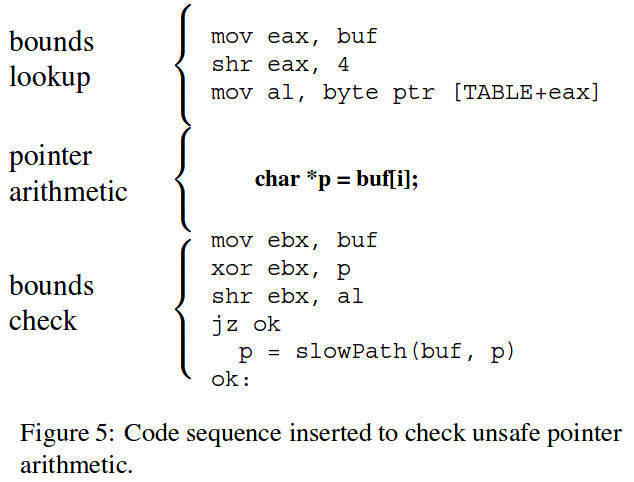
\includegraphics[width=0.6\textwidth]{../bounds/bb-bounds-check}
\end{frame}

\begin{frame}[fragile,label=addedCode]{baggy bounds check: added code}
    \lstset{language=myasm,style=small}
    \begin{lstlisting}
/* bounds lookup */
    mov buf, %rax
    shr %rax, 4
    mov LOOKUP_TABLE(%rax), %al
/* array element address computation */
    ...    // `\textbf{\textit{char * p = buf[i];}}`
/* bound check */
    mov buf, %rbx
    xor p, %rbx
    shr %al, %rbx
    jz  ok
    ...    // handle possible violation
ok:
\end{lstlisting}

    \imagecredit{adapted from paper figure}
\end{frame}

\begin{frame}{avoiding checks}
    \begin{itemize}
        \item code not added if not array/pointer accesses to object
        \item code not added when pointer accesses ``obviously'' safe
            \begin{itemize}
            \item author's implementation: only checked within function
            \end{itemize}
    \end{itemize}
\end{frame}



\subsection{exercise: overhead estimating?}
\begin{frame}<1>[fragile,label=bbOverheadExer1]{exercise: overhead of baggy bounds (1)}
\begin{itemize}
\item suppose program allocates:
    \begin{itemize}
    \item 1000 100 byte objects
    \item 1 10000 byte object
    \end{itemize}
\item using baggy bounds, estimate:
    \begin{itemize}
    \item space required for padding
        \begin{itemize}
        \item<2-> $(128-100)\cdot 1000 + (16384 - 10000)) = 34384$
        \end{itemize}
    \item space required for table
        \begin{itemize}
        \item<2-> $(128\cdot 1000 + 16384) \div 16 = 9024$
        \end{itemize}
    \end{itemize}
\end{itemize}
\end{frame}

\iftoggle{heldback}{}{\againframe<2>{bbOverheadExer1}}

\begin{frame}[fragile,label=bbOverheadExer2]{exercise: overhead of baggy bounds (2)}
\begin{lstlisting}[language=C,style=smaller]
char *strcat(char *d, char *s) {
    int i;
    for (i = 0; s[i] != '\0'; i += 1) {
        d[i] = s[i]; 
    }
    d[i] = '\0';
    return d;
}
\end{lstlisting}
\begin{itemize}
\item estimate:
\begin{itemize}
\item number of bounds checks needed
\item very rough number of instructions run w/o bounds check
\end{itemize}
\item thought question: \\
with bounds checking, what's fastest possible code?
\end{itemize}
\end{frame}


\subsection{alternative: pointer tagging}

\begin{frame}{alternate approach: pointer tagging}
    \begin{itemize}
        \item some bits of \myemph{address} are size 
        \begin{itemize}
        \item replaces table entry/lookup
        \end{itemize}
    \item change code to allocate objects this way
    \item works well on 64-bit --- plenty of addresses to use
    \end{itemize}
    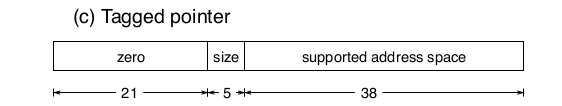
\includegraphics[width=0.8\textwidth]{../bounds/baggy-bounds-tagging}
\end{frame}



\subsection{performance?}

\begin{frame}{baggy bounds performance}
    \begin{itemize}
        \item table: 4--72\% time overhead (depends on benchmark suite)
        \item table: 11--21\% space overhead (depends on benchmark suite)
        \item tagged pointers: slightly better on average
    \end{itemize}
\end{frame}

\begin{frame}{baggy bounds performance}
    \begin{center}
    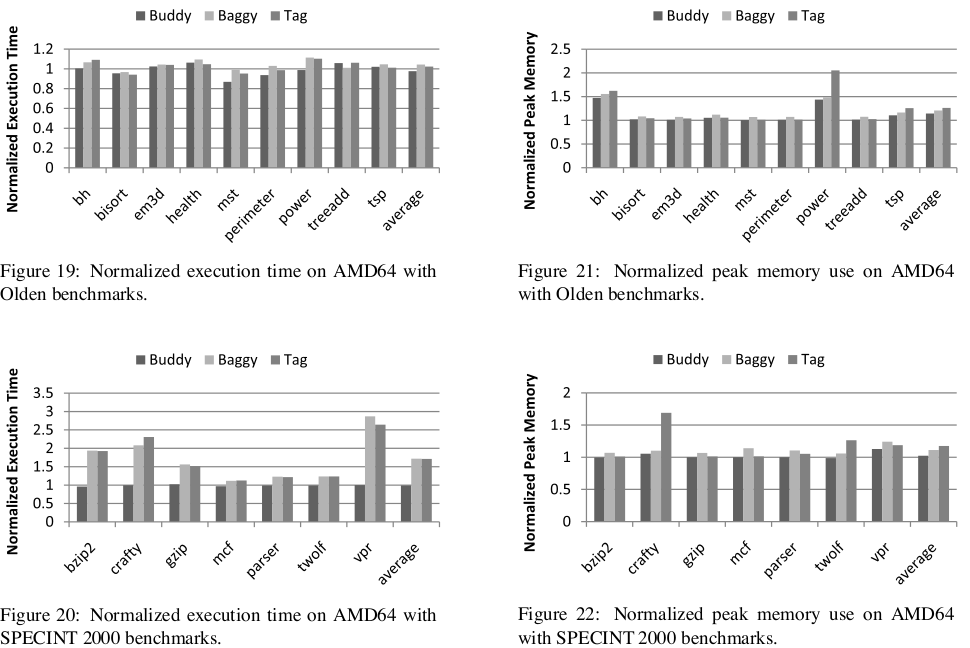
\includegraphics[height=0.8\textheight]{../bounds/baggy-bounds-perf}
    \end{center}
\end{frame}



\subsection{problem: pointers within objects}
% FIXME
\begin{frame}[fragile,label=withinObj]{problem: within object}
\begin{lstlisting}
struct foo {
    char buffer[1024];
    int *pointer;
};
struct foo array_of_foos[1024];
...
char *p = &array_of_foos[4].buffer[4]
\end{lstlisting}
\begin{itemize}
\item exercise: what are the bounds for p?
\end{itemize}
\end{frame}


\subsection{corner cases}

\begin{frame}[fragile,label=unfortunateCProgF2C]{unfortunate things C programmers do (4)}
in code generated by f2c (Fortran to C translator) \\
{\scriptsize (cleaned up slightly)}
\begin{lstlisting}[language=C,style=small]
float sum(int size, float *arr) {
    arr = arr - 1; /* <-- deliberately out-of-bounds pointer */
    float result = 0.f;
    for (i = 1; i <= size; ++i) {
        result += arr[i]
    }
    return result;
}
\end{lstlisting}
\end{frame}



\section{AddressSanitizer}

\begin{frame}{AddressSanitizer}
    \begin{itemize}
    \item like baggy bounds:
        \begin{itemize}
        \item big lookup table
        \item lookup table set by memory allocations
        \item compiler modification: change stack allocations
        \end{itemize}
    \item unlike baggy bounds:
        \begin{itemize}
        \item check reads/writes (instead of pointer computations)
        \item only detect errors that read/write \myemph{between objects}
        \item object sizes not padded to power of two
        \item table has info for every single byte (more precise)
        \end{itemize}
    \end{itemize}
\end{frame}




\subsection{ASan's added check}

\begin{frame}[fragile,label=asanVBounds]{adding bounds-checking example}
\lstset{
    language=C++,
    style=small,
    moredelim={**[is][\btHL<2>]{~2~}{~end~}},
}
\begin{lstlisting}
void vulnerable(long value, int offset) {
    long array[10] = {1,2,3,4,5,6,7,8,9,10};
    // generated code: (added by AddressSanitizer)
    ~2~if (!lookup_table[&array[offset]] == VALID) FAIL();~end~
    array[offset] = value;
    do_something_with(array);
}
\end{lstlisting}
    \begin{itemize}
        \item AddressSanitizer: crashes only if \lstinline|array[offset]| isn't part of any object
            \begin{itemize}
            \item but no extra space --- single-byte precision
            \end{itemize}
    \end{itemize}
\end{frame}



\subsection{stack layout}
\usetikzlibrary{arrows.meta,matrix,patterns}
\tikzset{
    stackBox/.style={very thick},
    allocBox/.style={dashed,very thick,fill=blue!20},
    onStack/.style={thick},
    frameOne/.style={fill=blue!15},
    frameTwo/.style={fill=red!15},
    markLine/.style={blue!50!black},
    markLineB/.style={red!90!black},
    hiLine/.style={red!90!black},
}
\begin{frame}[fragile,label=asanStackLayout]{AddressSanitizer stack layout}
    \begin{tikzpicture}
        \begin{scope}[x=1.7cm]
    \draw[stackBox] (0, 0) rectangle (5, -6);
            \draw[onStack] (0, 0) rectangle (5, -.5)
        node[midway] (arrayLoc) { return address (for \texttt{vulernable()}) };
    \begin{visibleenv}<2>
        \node[anchor=west] at (5.25, -.25) { $\approx$ \tt array[0x13]};
        \node[anchor=west] at (5.25, -3.75) { $\approx$ \tt array[0xa]};
    \end{visibleenv}
    \draw[onStack] (0, -.5) rectangle (5, -1)
        node[midway] { saved \tt\%rbp };
    \draw[onStack] (0, -1) rectangle (5, -1.5)
        node[midway] { saved \tt\%r13 };
    \draw[onStack] (0, -1.5) rectangle (5, -2)
        node[midway] { saved \tt\%r12 };
    \draw[onStack] (0, -2) rectangle (5, -2.5)
        node[midway] { saved \tt\%rbx };
    \draw[onStack,pattern=north west lines,pattern color=red] (0, -2.5) rectangle (5, -4)
        node[midway,fill=white] { ``red zone'' };
    \draw[onStack] (0, -4) rectangle (5, -6)
        node[midway,fill=white] { \tt array };
            \draw[onStack,dashed] (0, -4) rectangle (5, -4.5) node[midway] {\tt array[9]};
            \begin{visibleenv}<3>
            \matrix[tight matrix,
                nodes={text width=3cm,font=\small\tt},anchor=north west,label={north:lookup table}] (tbl) at (6, -2) {
                valid \\ valid  \\ valid \\ valid \\ valid \\ invalid \\ invalid \\
                invalid \\ invalid \\ valid \\ valid \\ \ldots \\
            };
                \draw[thick,-Latex] (5, -.25) -- (tbl-1-1.west);
                \draw[thick,-Latex] (5, -.75) -- (tbl-2-1.west);
            \end{visibleenv}
    \draw[thick,-Latex] (5.15, -6) --++ (0, 2);
        \end{scope}
    \end{tikzpicture}
\end{frame}





\end{document}
